\chapter{Covariance matrixes}\label{app:Cor}
The covariance matrix of cross sections measurements is calculated as:
\begin{equation}
C_{XY}=\sum_{k}\sigma^k_X\sigma^k_Y \rho^{k}_{XY},
\end{equation}
where index $k$ runs over all independent sources of uncertainties, $\sigma^k_X$ and $\sigma^k_Y$ are the $k$-th uncertainties of the measurement X and Y respectively. The coefficient $\rho^k_{XY}$ - is a correlation coefficient between two estimates from the correlation matrix. Each element of the diagonal matrix is equal to 1. The off-diagonal elements are equal to 0 for non correlated sources of uncertainty, to 1 for totally correlated and -1 for totally uncorrelated. The uncertainties sources and their correlations are explained in Chap.~\ref{chap:Unc}.

The covariance matrix for the cross-section measurements in electron and muon channels are shown in Fig.~\ref{fig:AppCE}-~\ref{fig:AppCMu}. The correlation matrix for the combined measurement is shown in Fig.~\ref{fig:AppCComb}. The correlation matrix of the ratios $R_W$ and $R_Z$ used in Sec.~\ref{sec:LeptUnivers} is shown in Fig.~\ref{fig:AppCR}.


\begin{figure}[!h]
\begin{minipage}[h]{0.32\linewidth}
\center{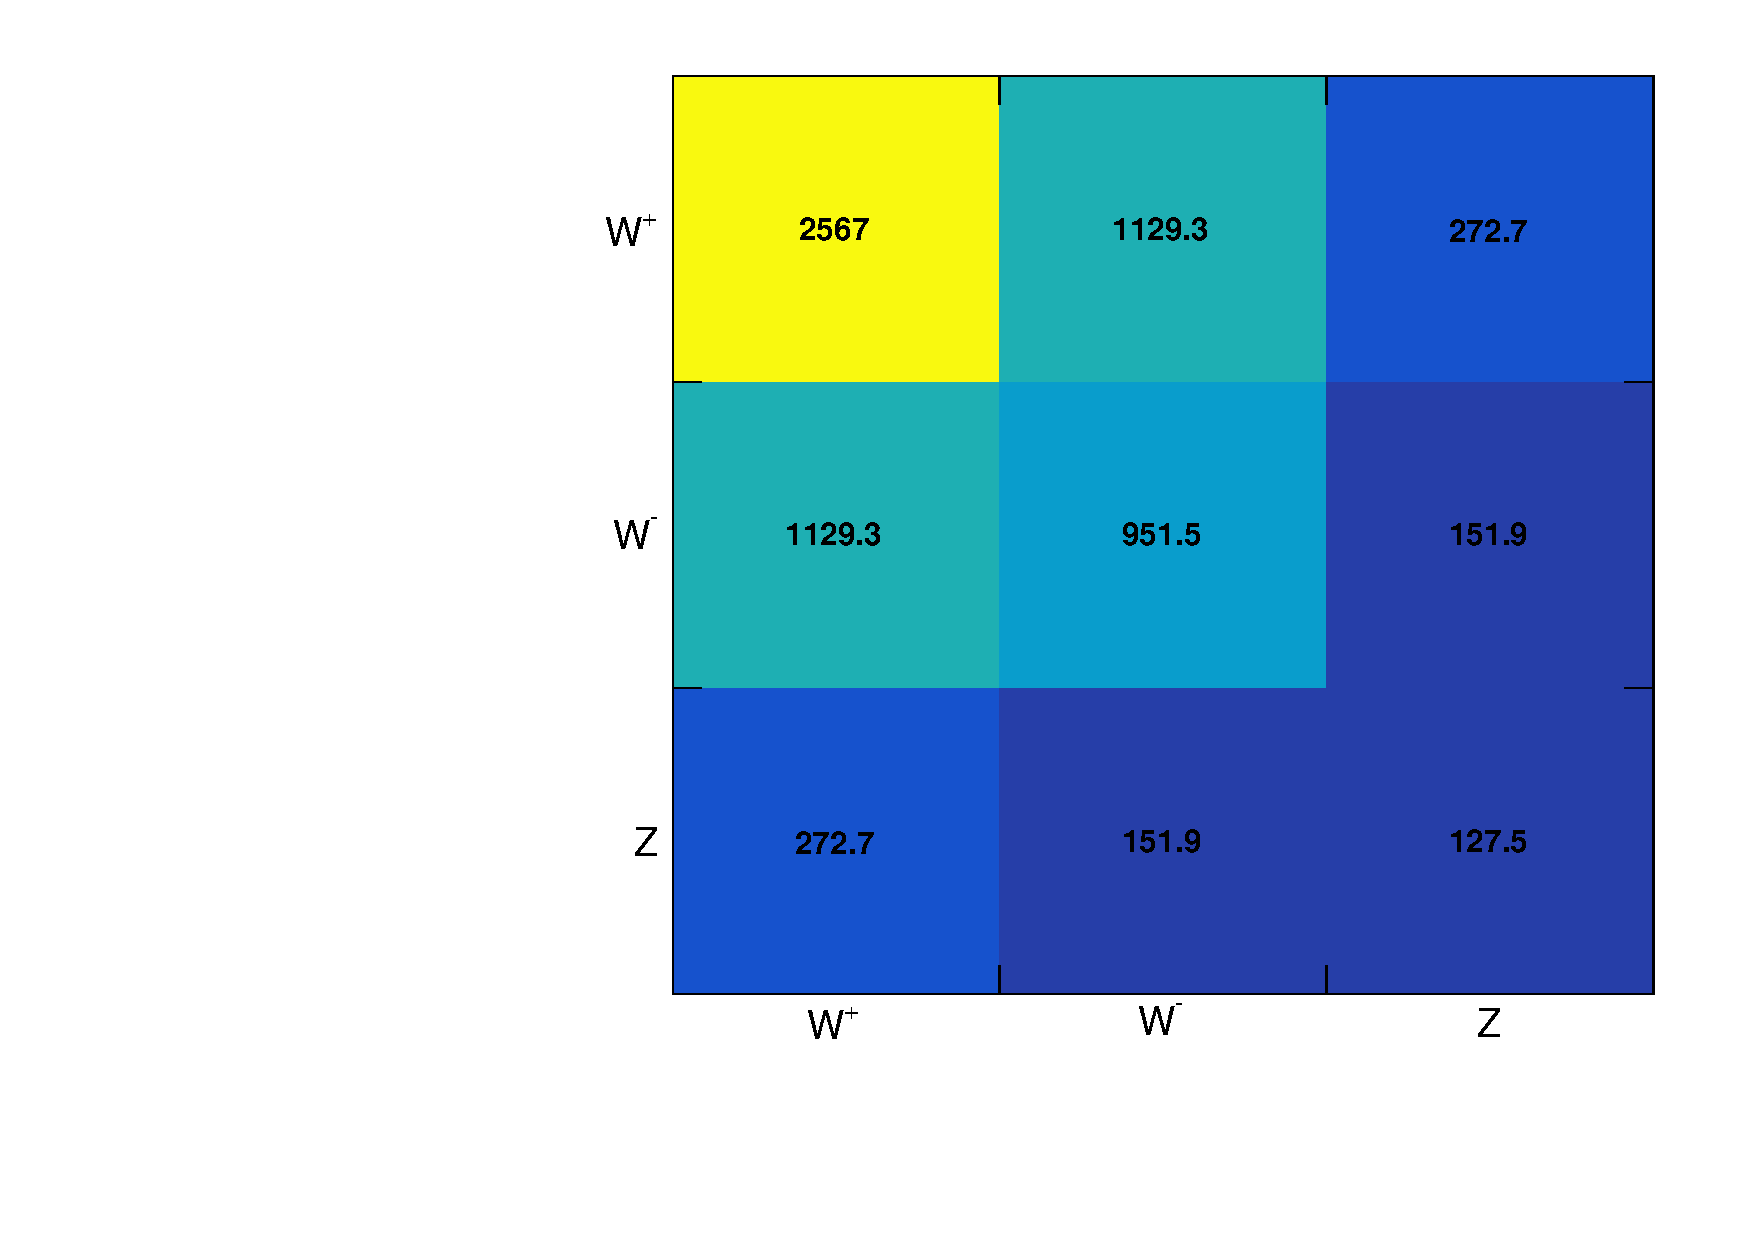
\includegraphics[width=1\textwidth]{Results/CovEnu0.pdf} \\ c)}
\end{minipage}
\hfill
\begin{minipage}[h]{0.32\linewidth}
\center{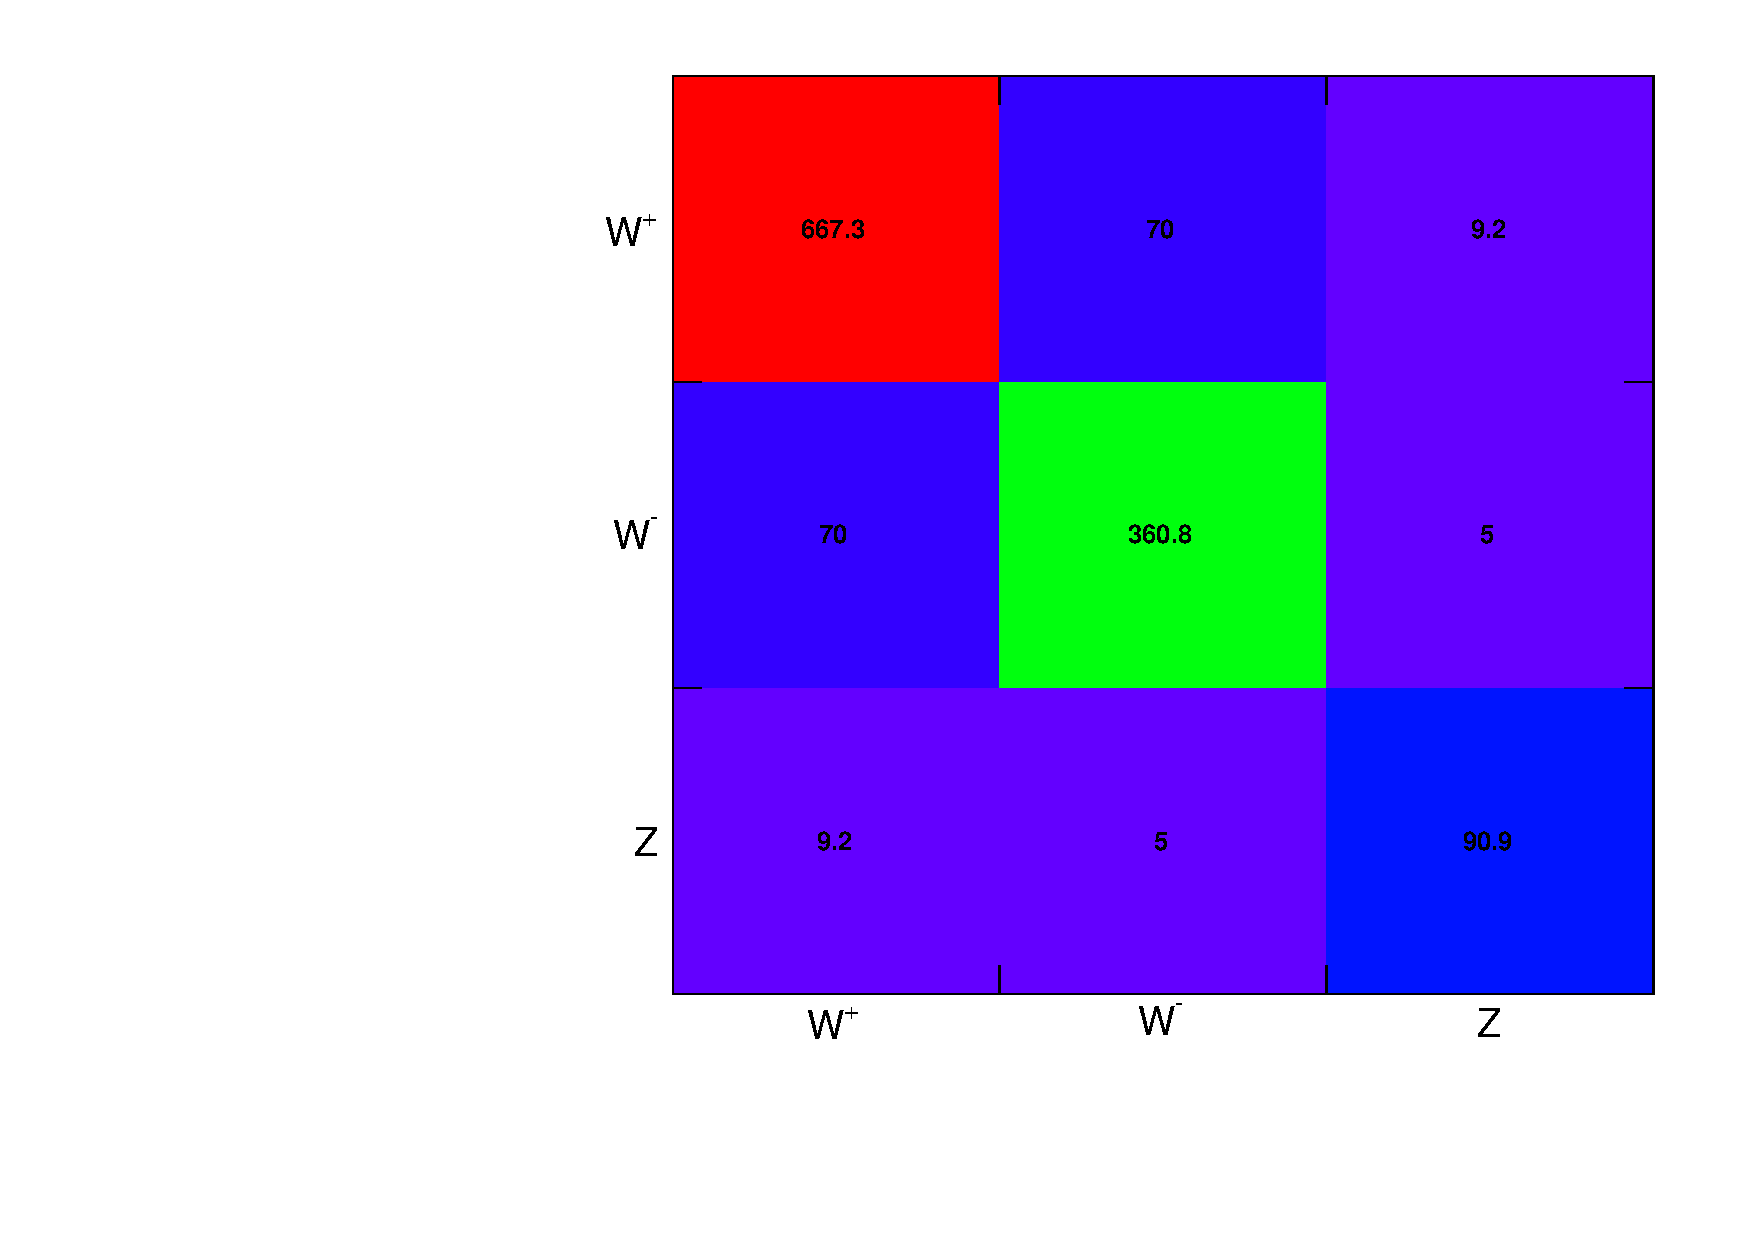
\includegraphics[width=1\textwidth]{Results/CovEnu1.pdf} \\ b)}
\end{minipage}
\hfill
\begin{minipage}[h]{0.32\linewidth}
\center{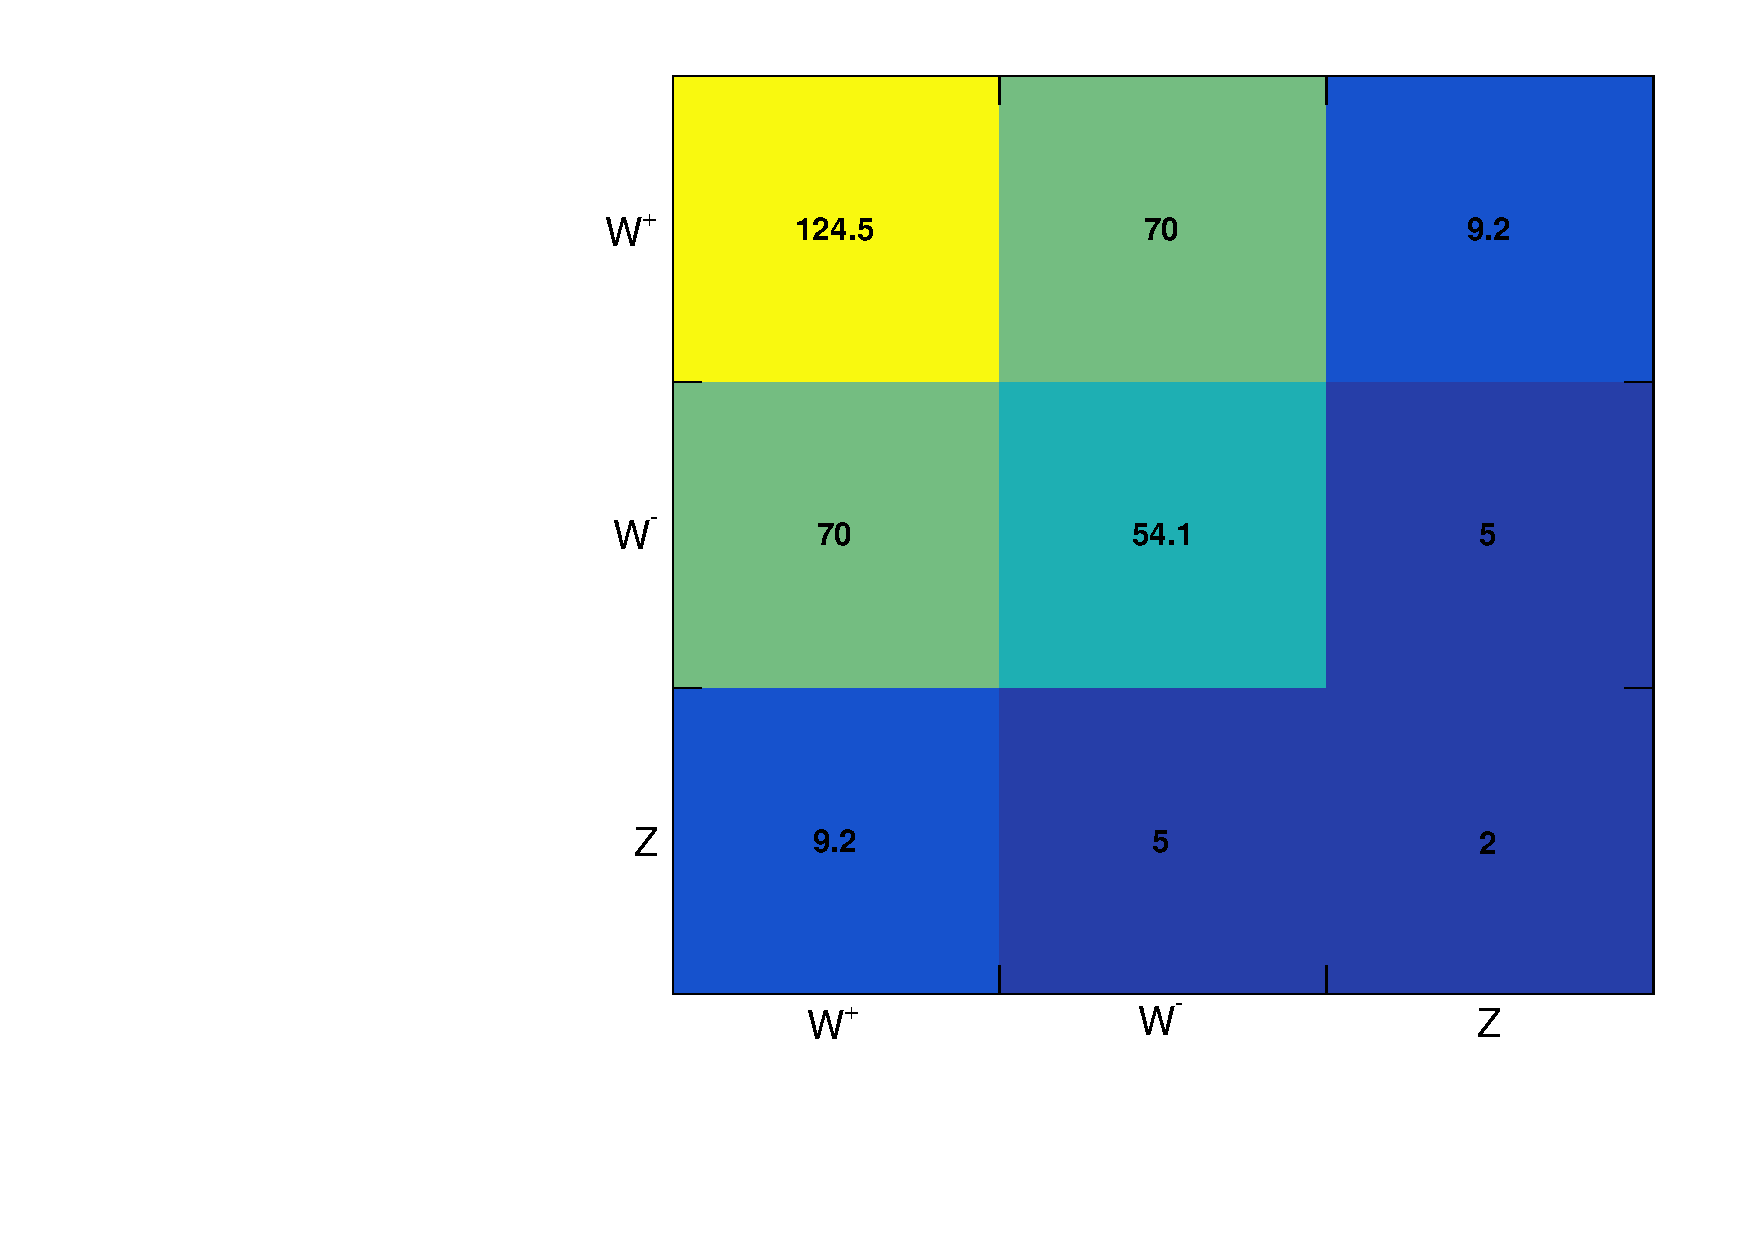
\includegraphics[width=1\textwidth]{Results/CovEnu2.pdf} \\ c)}
\end{minipage}
\caption{Covariance matrix for the measurements of $Z$, $W^+$ and $W^{-}$  cross sections for electron channel in fiducial region a) for all uncertainty b) for all but luminosity uncertainty c) for all but luminosity and statistical uncertainty. }
\label{fig:AppCE}
\end{figure}

\begin{figure}[!h]
\begin{minipage}[h]{0.32\linewidth}
\center{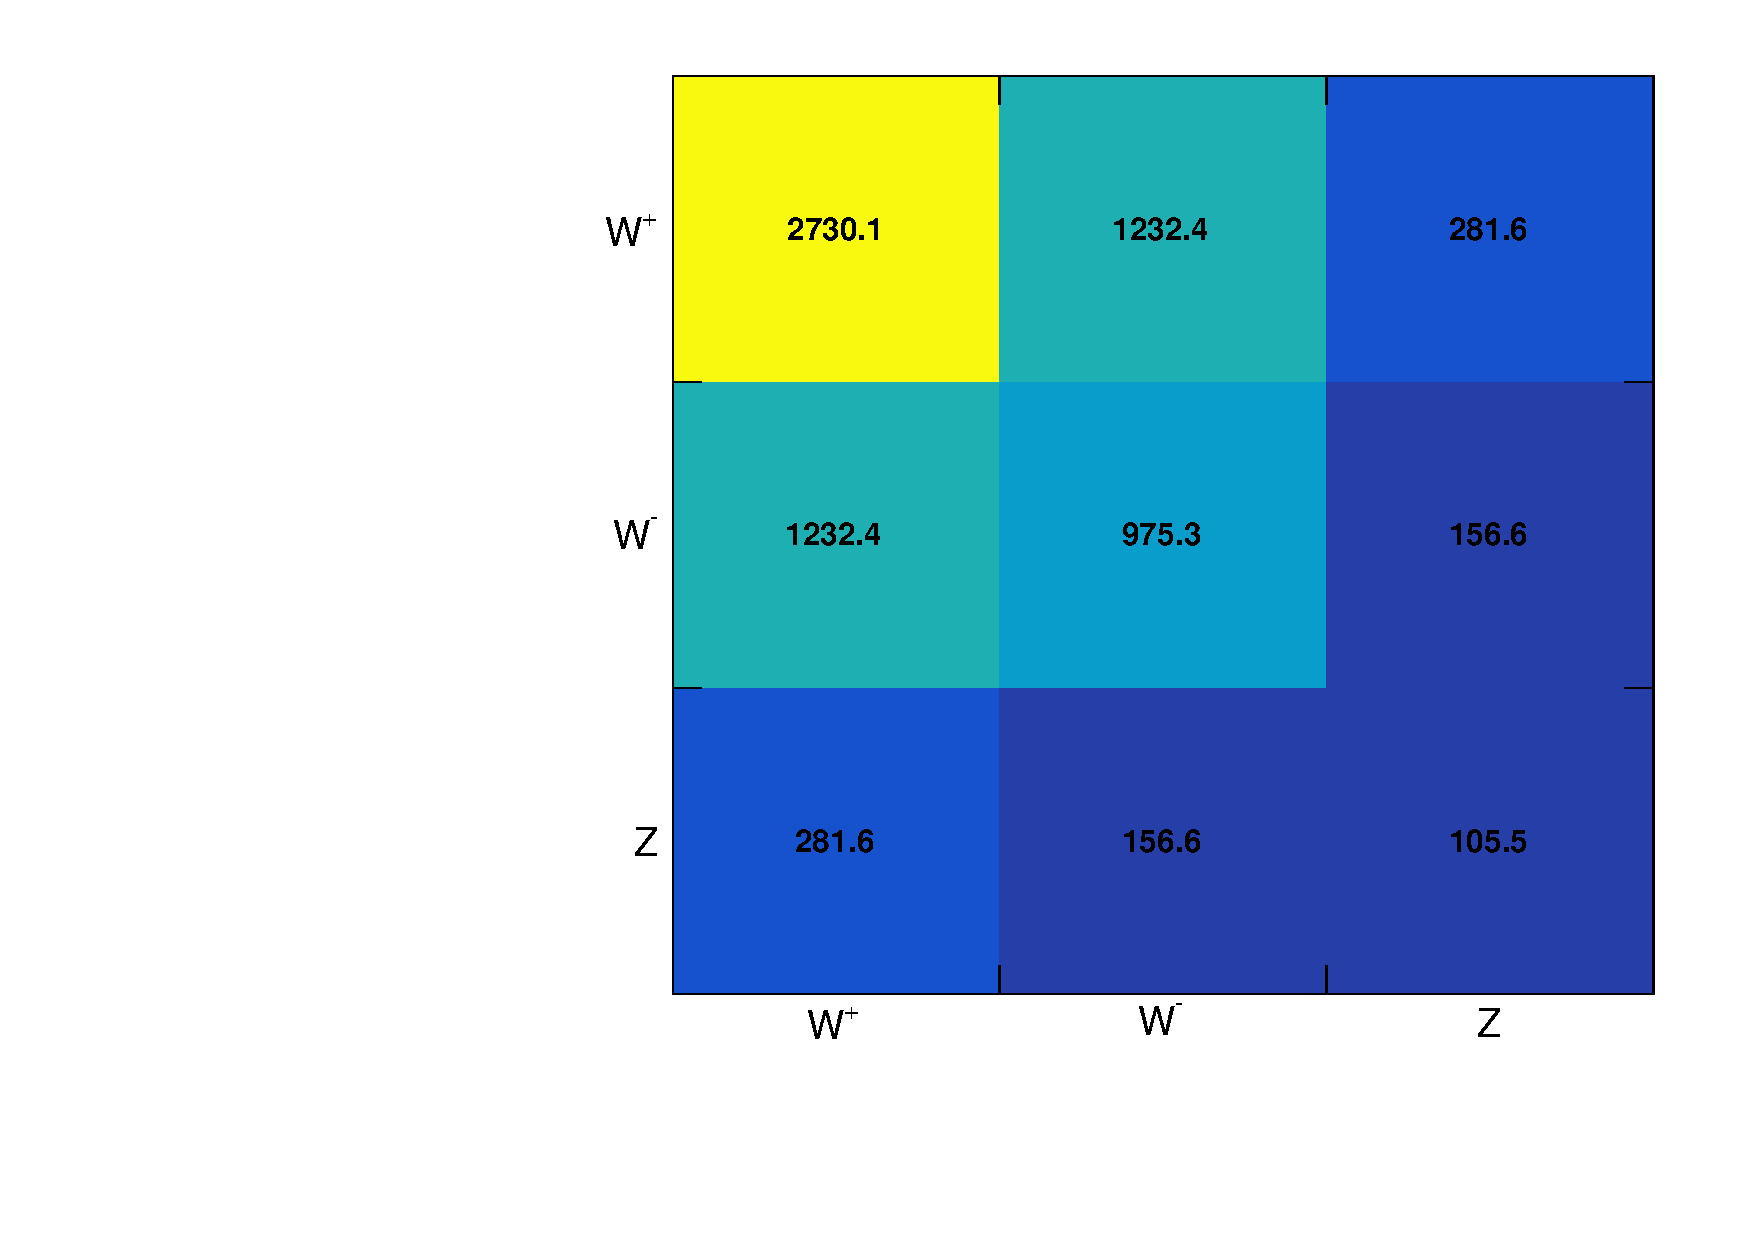
\includegraphics[width=1\textwidth]{Results/CovMunu0.pdf} \\ c)}
\end{minipage}
\hfill
\begin{minipage}[h]{0.32\linewidth}
\center{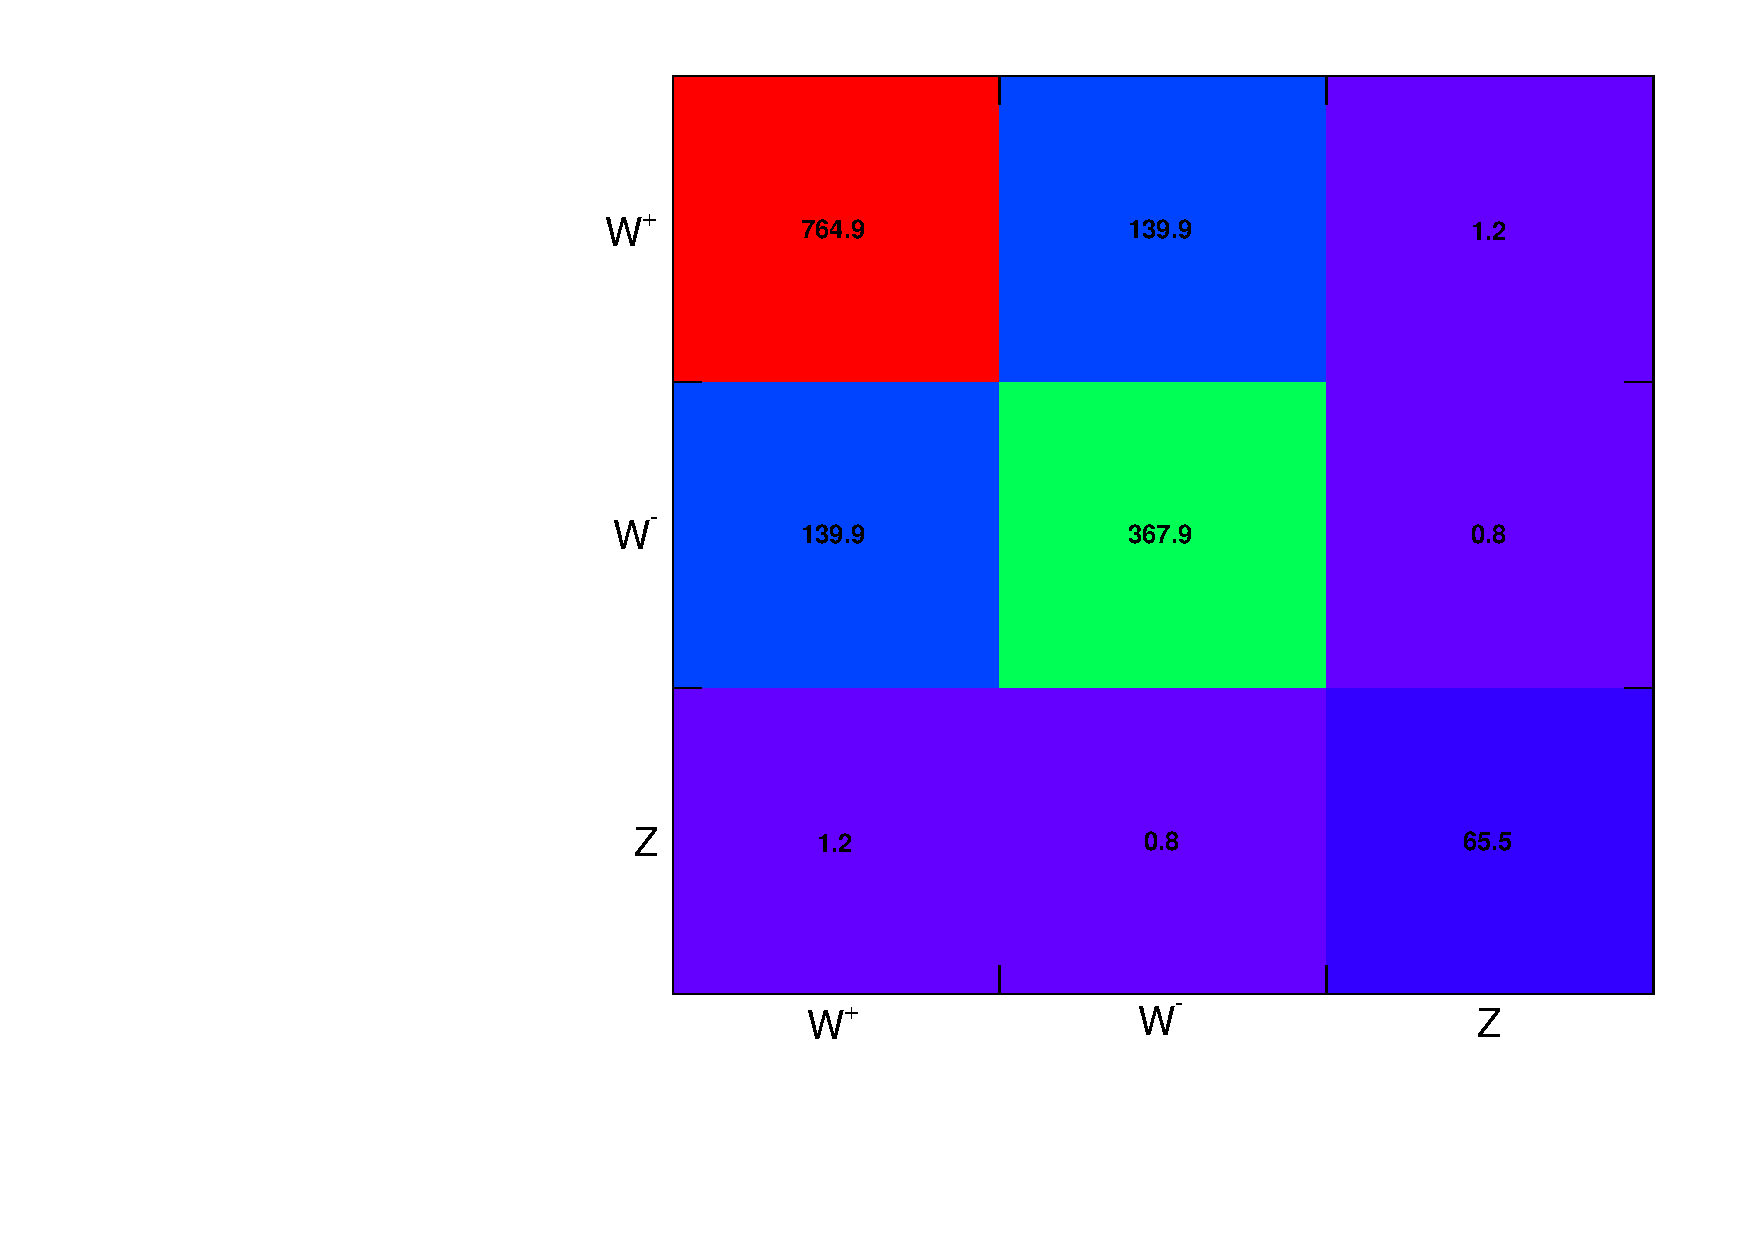
\includegraphics[width=1\textwidth]{Results/CovMunu1.pdf} \\ b)}
\end{minipage}
\hfill
\begin{minipage}[h]{0.32\linewidth}
\center{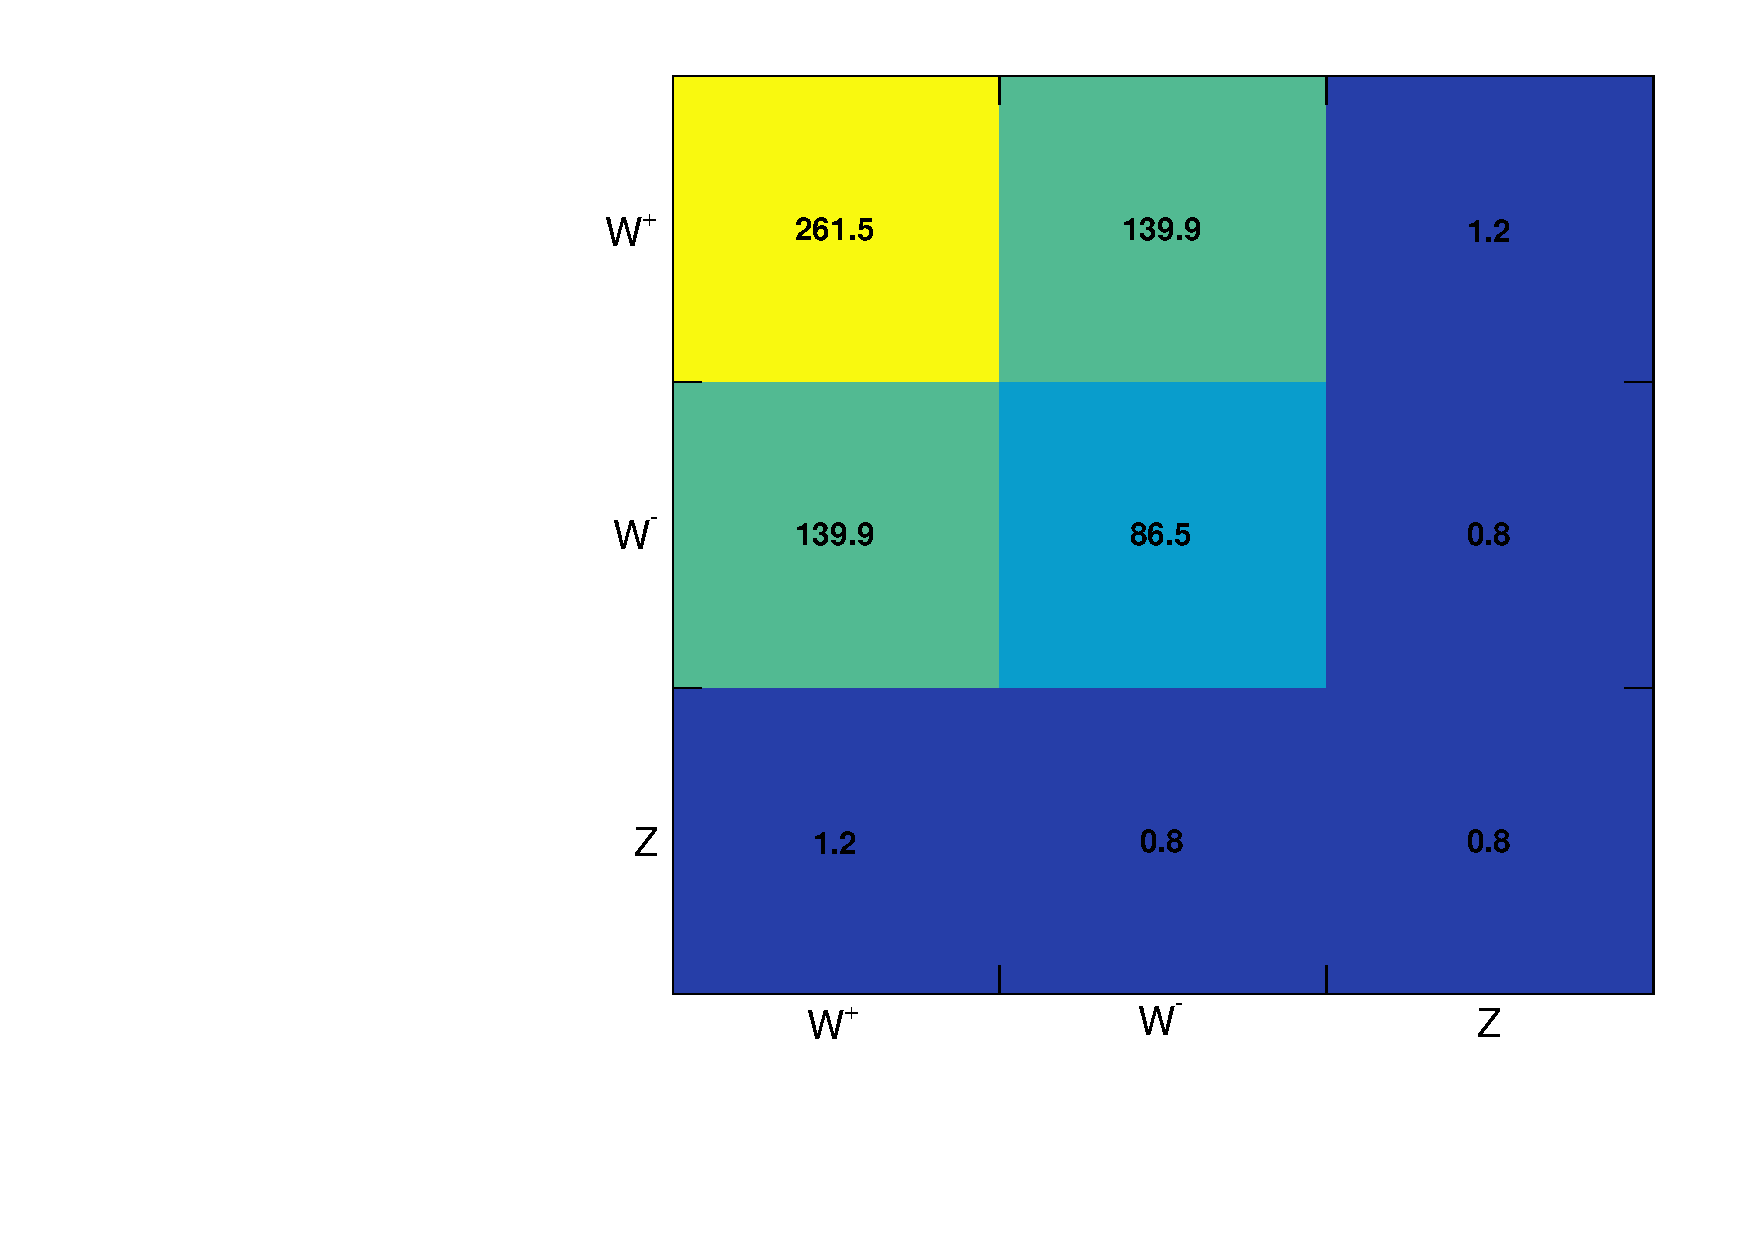
\includegraphics[width=1\textwidth]{Results/CovMunu2.pdf} \\ c)}
\end{minipage}
\caption{Covariance matrix for the measurements of $Z$, $W^+$ and $W^{-}$  cross sections for muon channel in fiducial region a) for all uncertainty b) for all but luminosity uncertainty c) for all but luminosity and statistical uncertainty. }
\label{fig:AppCMu}
\end{figure}


\begin{figure}[!h]
\begin{minipage}[h]{0.32\linewidth}
\center{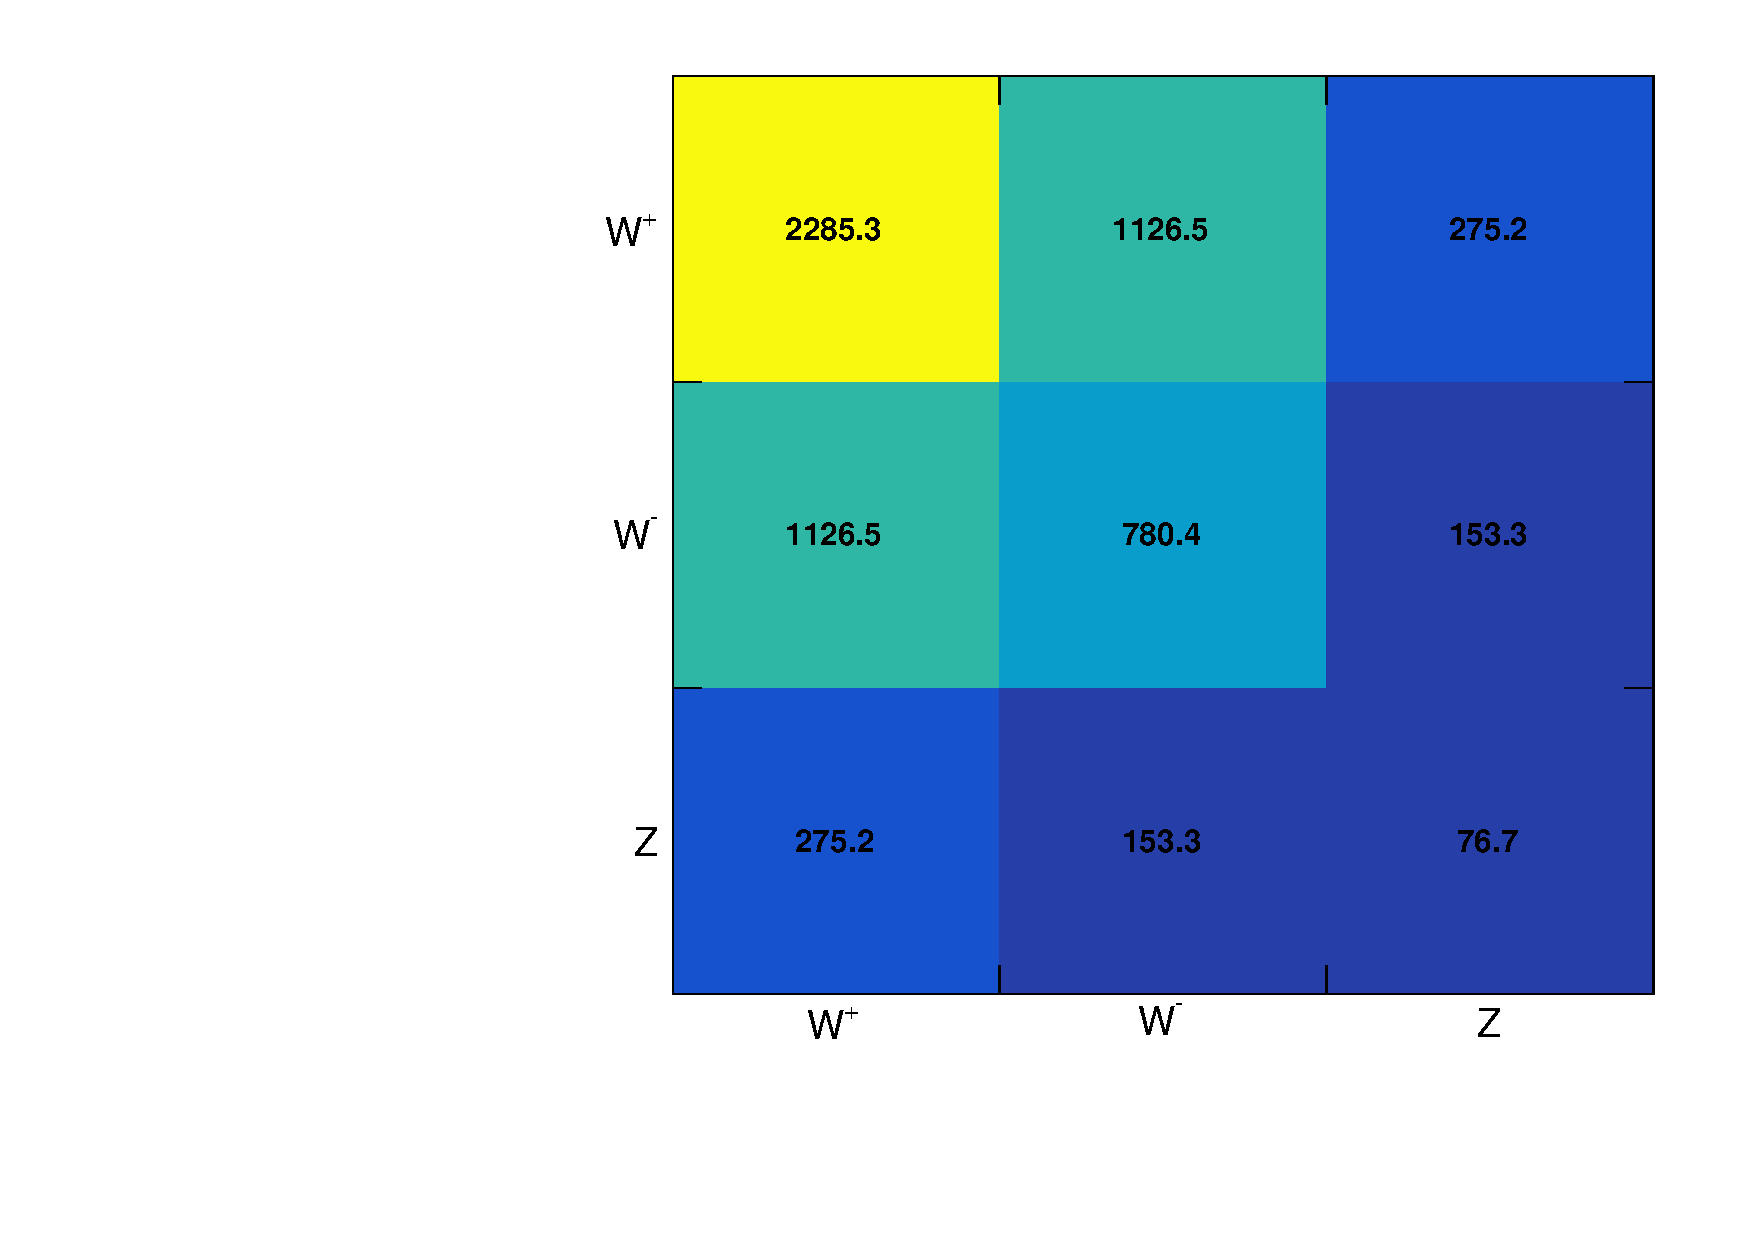
\includegraphics[width=1\textwidth]{Results/CovTot0.pdf} \\ c)}
\end{minipage}
\hfill
\begin{minipage}[h]{0.32\linewidth}
\center{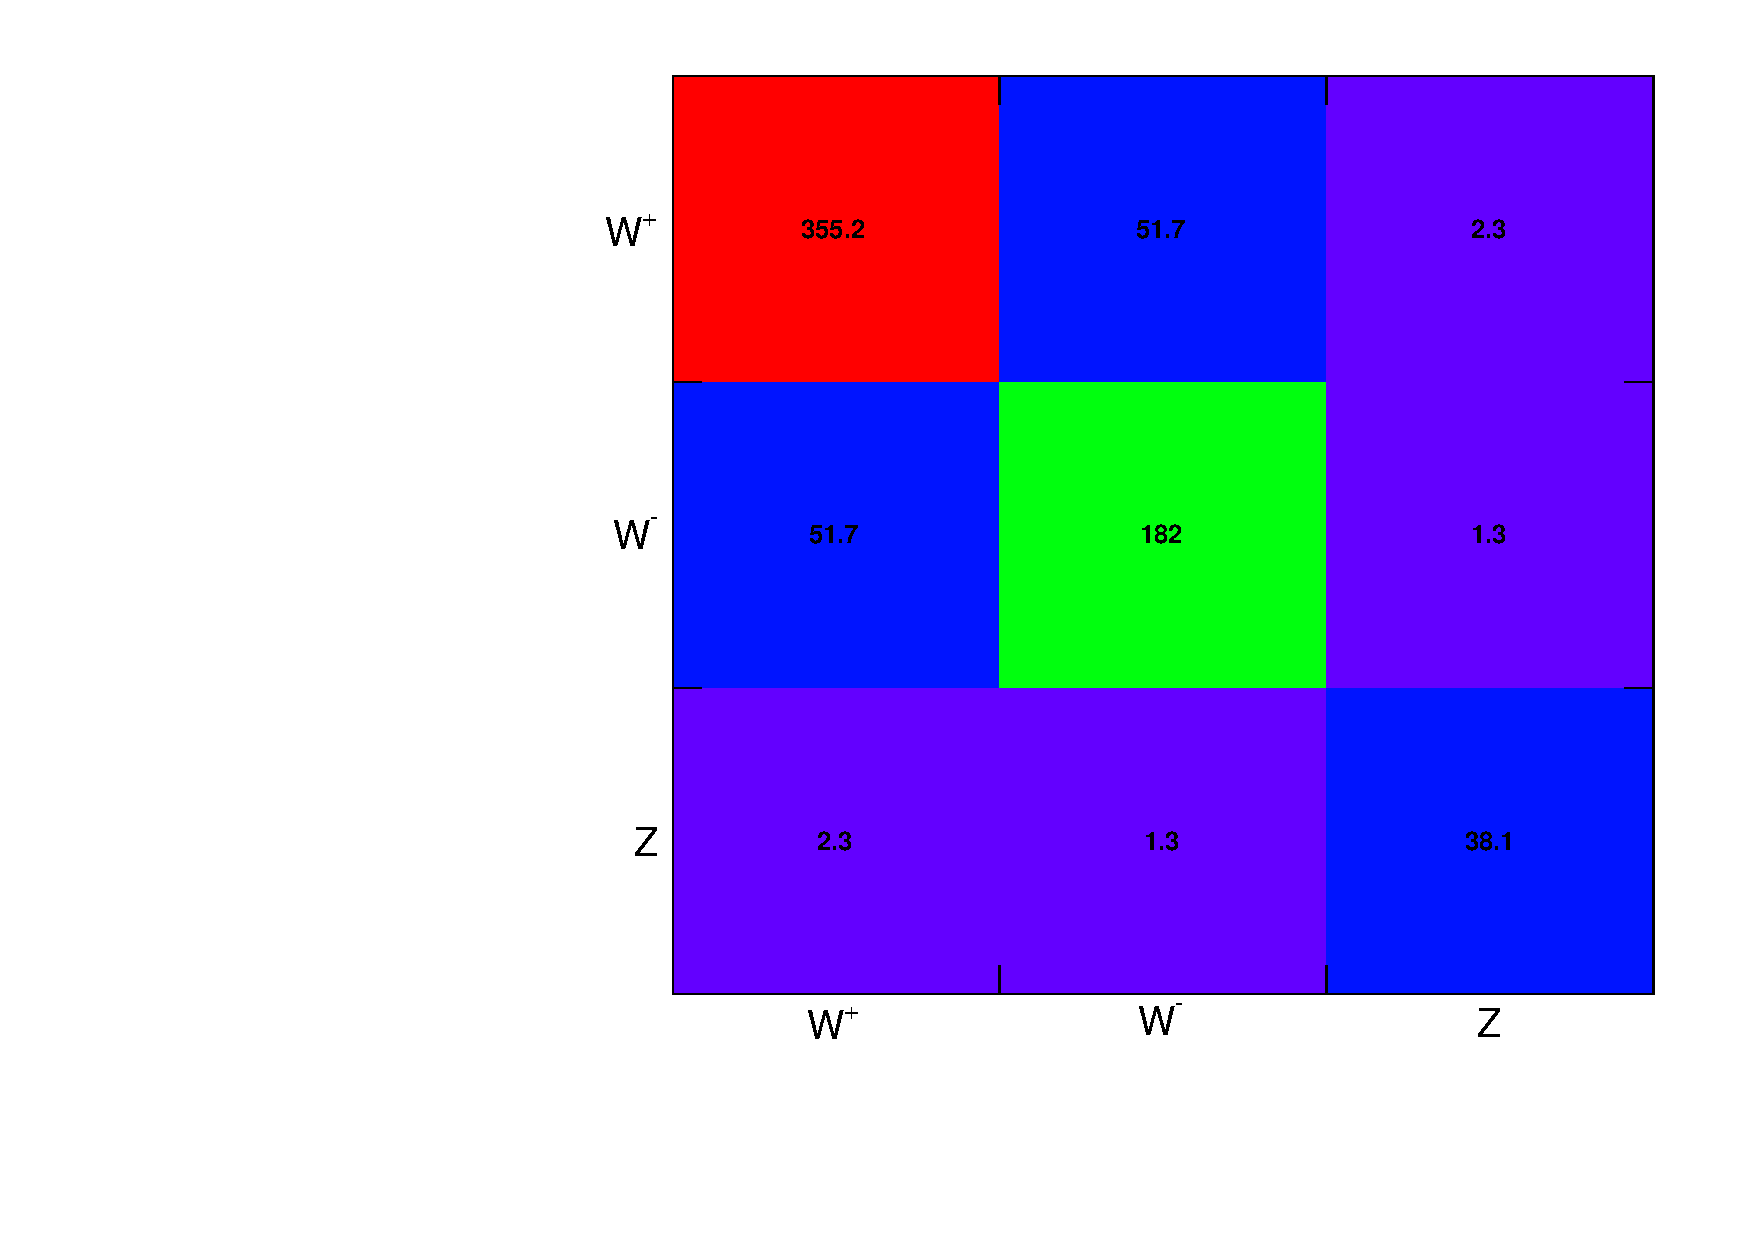
\includegraphics[width=1\textwidth]{Results/CovTot1.pdf} \\ b)}
\end{minipage}
\hfill
\begin{minipage}[h]{0.32\linewidth}
\center{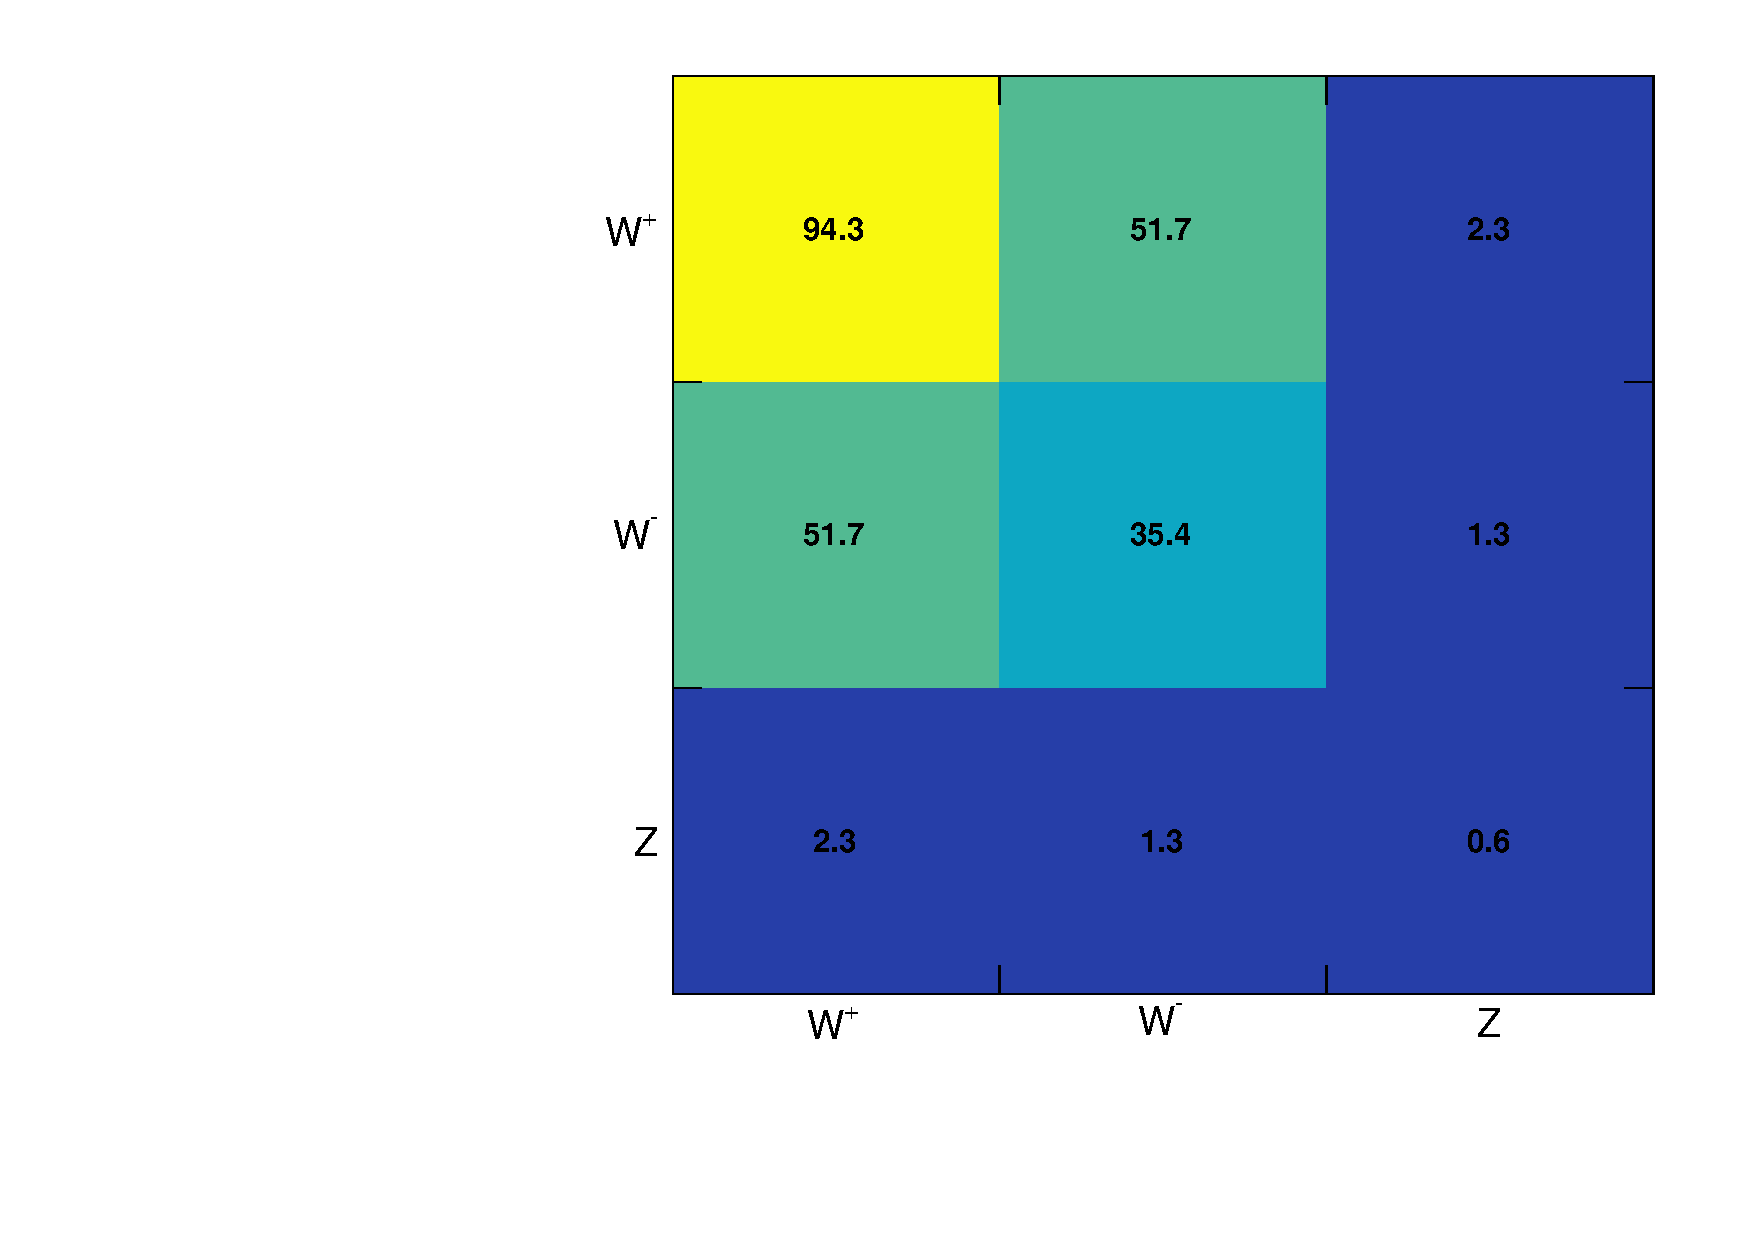
\includegraphics[width=1\textwidth]{Results/CovTot2.pdf} \\ c)}
\end{minipage}
\caption{Covariance matrix for the measurements of $Z$, $W^+$ and $W^{-}$  cross sections for combined channel in fiducial region a) for all uncertainty b) for all but luminosity uncertainty c) for all but luminosity and statistical uncertainty. }
\label{fig:AppCComb}
\end{figure}

\begin{figure}[!h]
\begin{minipage}[h]{0.49\linewidth}
\center{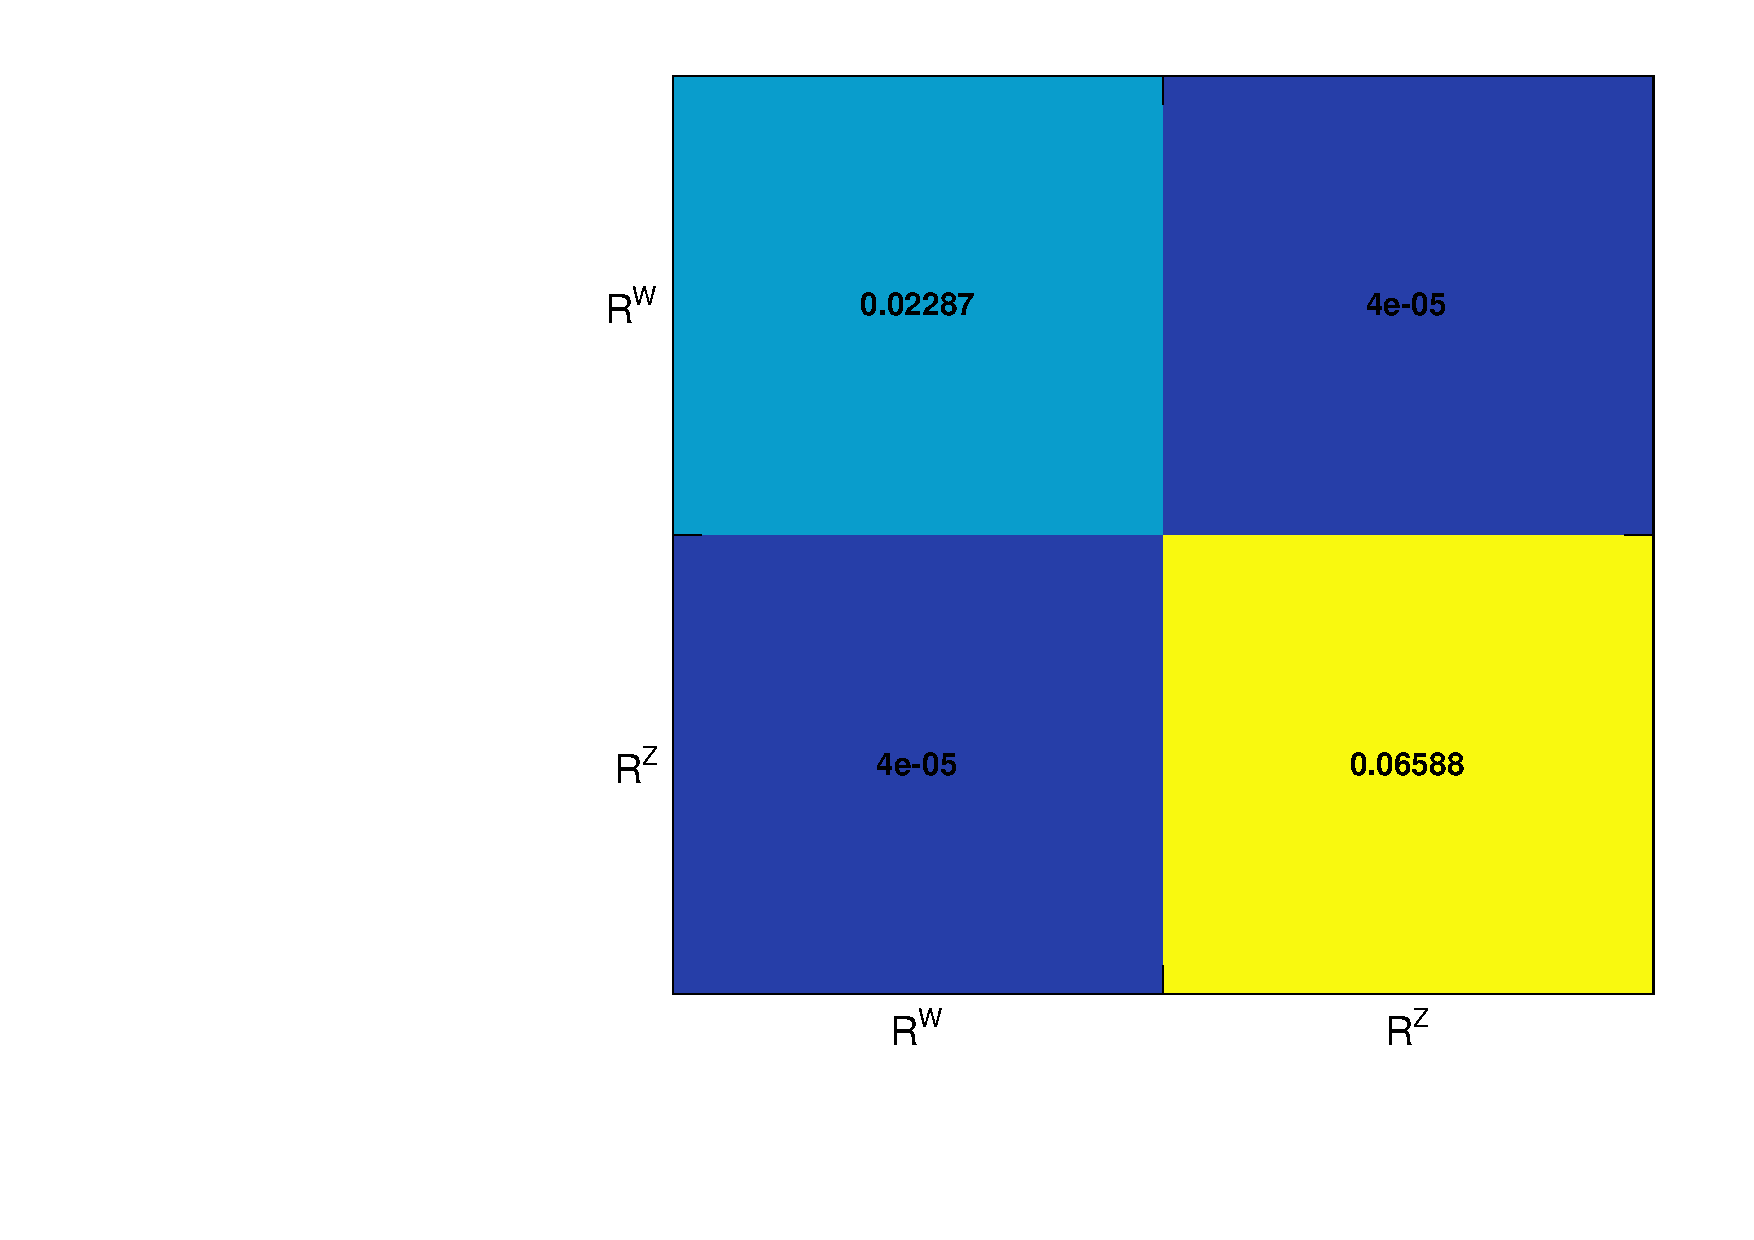
\includegraphics[width=1\textwidth]{Results/CovUniversWithStat.pdf} \\ c)}
\end{minipage}
\hfill
\begin{minipage}[h]{0.49\linewidth}
\center{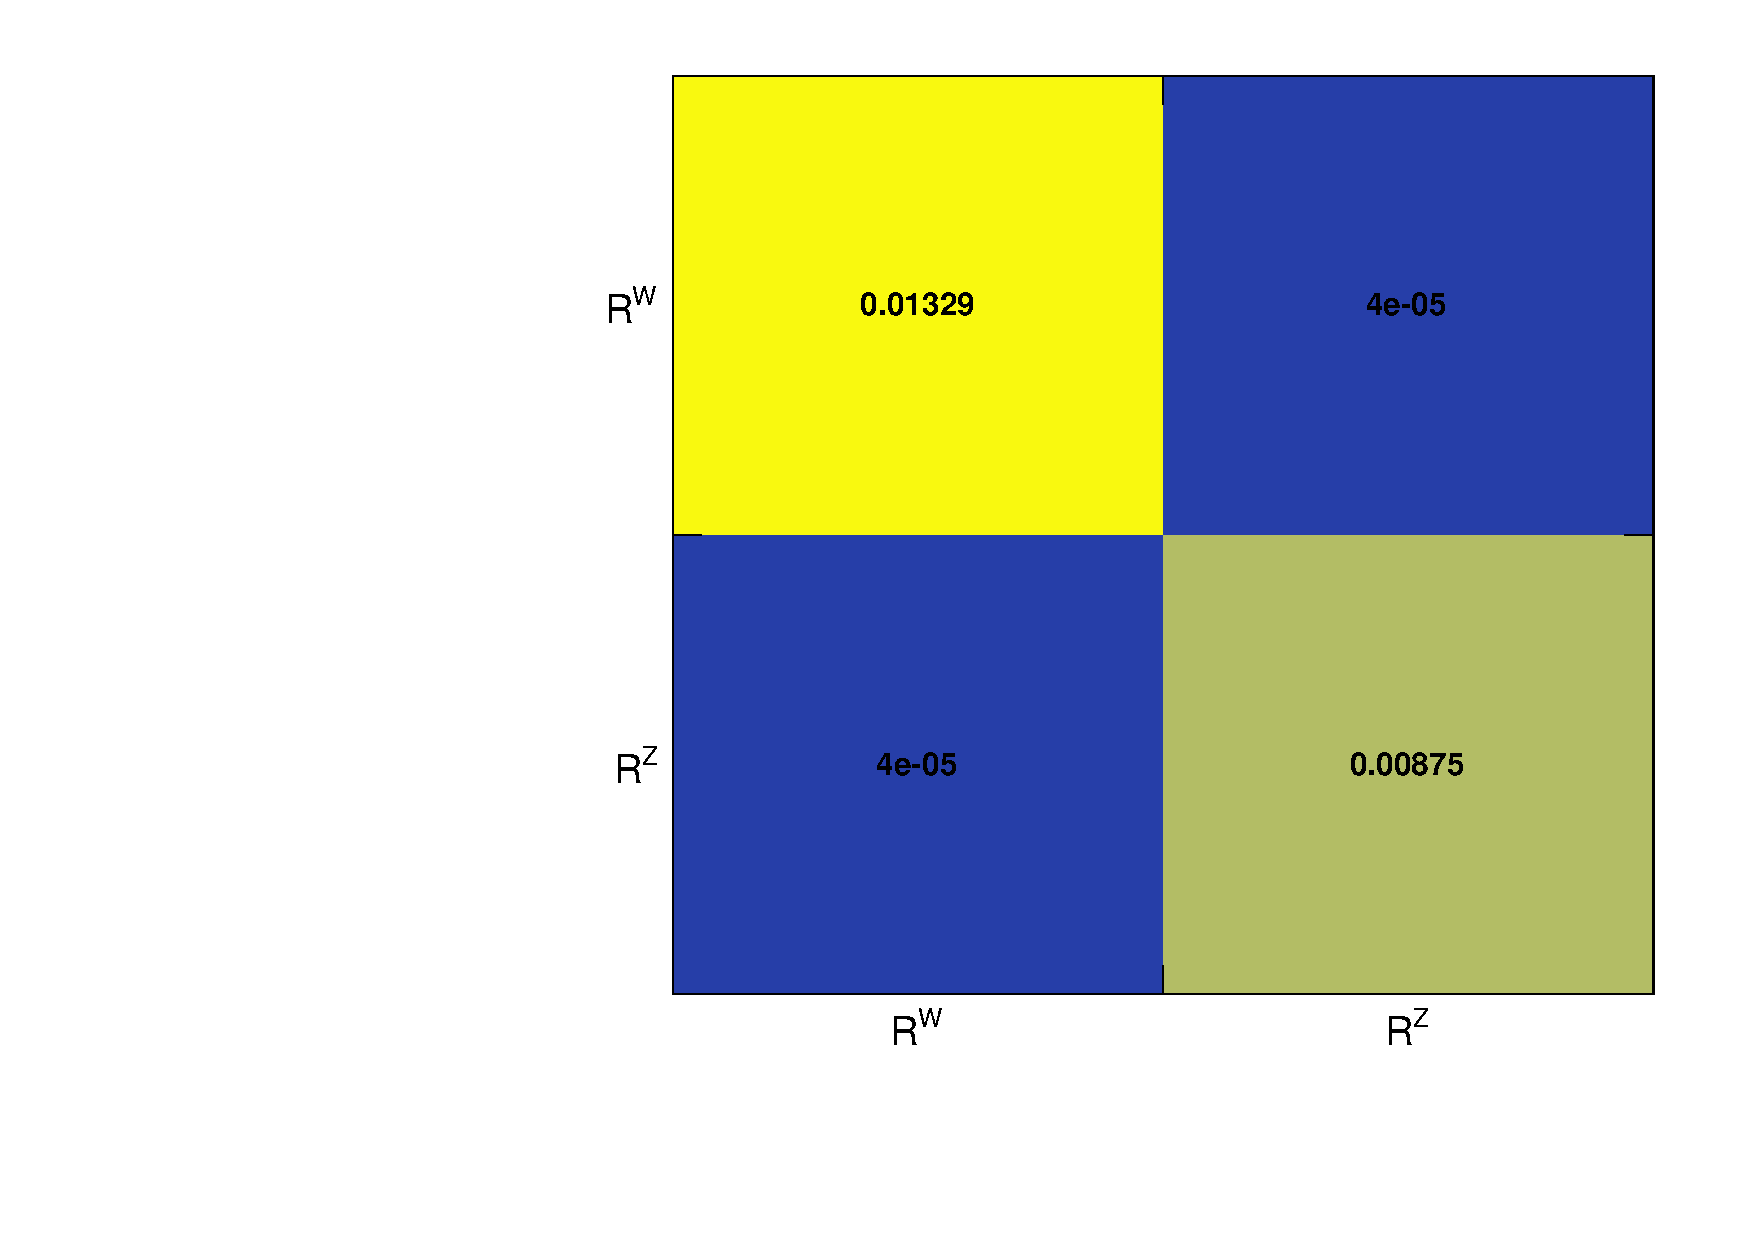
\includegraphics[width=1\textwidth]{Results/CovUniversNoStat.pdf} \\ b)}
\end{minipage}
\caption{Covariance matrix for the measurements of $R_{W}$ and $R_{Z}$  ratios from Sec.~\ref{sec:LeptUnivers} for electron channel in fiducial region a) for all uncertainty b)for all but statistical uncertainty. }
\label{fig:AppCR}
\end{figure}
